\documentclass[pageno]{jpaper}

%replace XXX with the submission number you are given from the ISCA submission site.
\newcommand{\IWreport}{2015}

\usepackage[normalem]{ulem}
\usepackage{array}
\usepackage{amsmath}
\usepackage{tabu}
\usepackage{relsize}
\usepackage{float}
\usepackage{longtable}

\begin{document}

\title{
Predicting Stock Price Direction using Support Vector Machines}
\author{Saahil Madge \\ Advisor: Professor Swati Bhatt}

\date{}
\maketitle

\thispagestyle{empty}

\begin{abstract}
\bigskip
Support Vector Machine is a machine learning technique used in recent studies to forecast stock prices. This study uses daily closing prices for 34 technology stocks to calculate price volatility and momentum for individual stocks and for the overall sector. These are used as parameters to the SVM model. The model attempts to predict whether a stock price sometime in the future will be higher or lower than it is on a given day. We find little predictive ability in the short-run but definite predictive ability in the long-run.
\end{abstract}

\section{Introduction}

Stock price prediction is one of the most widely studied and challenging problems, attracting researchers from many fields including economics, history, finance, mathematics, and computer science. The volatile nature of the stock market makes it difficult to apply simple time-series or regression techniques. Financial institutions and traders have created various proprietary models to try and beat the market for themselves or their clients, but rarely has anyone achieved consistently higher-than-average returns on investment. Nevertheless, the challenge of stock forecasting is so appealing because an improvement of just a few percentage points can increase profit by millions of dollars for these institutions.

Traditionally, many prediction models have focused on linear statistical time series models such as ARIMA \cite{bontempi}. However, the variance underlying the movement of stocks and other assets makes linear techniques suboptimal, and non-linear models like ARCH tend to have lower predictive error \cite{zhang}. Recently, researchers have turned to techniques in the computer science fields of big data and machine learning for stock price forecasting. These apply computational power to extend theories in mathematics and statistics. Machine learning algorithms use given data to ``figure out'' the solution to a given problem. Big data and machine learning techniques are also the basis for algorithmic and high-frequency trading routines used by financial institutions.

In this paper we focus on a specific machine learning technique known as Support Vector Machines (SVM). Our goal is to use SVM at time $t$ to predict whether a given stock's price is higher or lower on day $t+m$. We look at the technology sector and 34 technology stocks in particular. We input four parameters to the model - the recent price volatility and momentum of the individual stock and of the technology sector. These parameters are calculated using daily closing prices for each stock from the years 2007 through 2014. We analyze whether this historical data can help us predict price direction. If the Efficient Markets Hypothesis (EMH) holds true, prices should follow a random walk and be unpredictable based on historical data. We find that in the short-term this holds true, but in the long-term we are able to reach prediction accuracies between 55\% and 60\%. We conclude that our model is able to achieve significant prediction accuracies with some parameters in the long-term, but that we must look at more granular intra-day trading data to achieve prediction accuracies in the short-term.

\section{Background Information}
\subsection{Stock Market Efficiency}
\label{subsec: stock}
Much economic research has been conducted into the {\em Efficient Markets Hypothesis} theory, which posits that stock prices already reflect all available information \cite{bodie} and are therefore unpredictable. According to the EMH, stock prices will only respond to new information and so will follow a random walk. If they only respond to new information, they cannot be predicted. That the stocks follow a random walk is actually a sign of market efficiency, since predictable movement would mean that information was not being reflected by the market prices.

There are three variants of this theory -- weak, semi-strong, and strong. Most research has concluded that the semi-strong version holds true. This version claims that stock prices reflect all {\em publicly} available information, but private information can be used to unfairly predict profits. This is the basis behind severe insider trading laws.

Nevertheless, there are certain market phenomena that actually run contrary to EMH. These are known as market anomalies. Jegadeesh and Titman discovered that in the short term, stock prices tend to exhibit momentum\cite{jegadeesh}. Stocks that have recently been increasing continue to increase, and recently decreasing stocks continue to decrease. This type of trend implies some amount of predictability to future stock prices, contradicting the EMH. 

The stock market also exhibits seasonal trends. Jacobsen and Zhang studied centuries' worth of data and found that trading strategies can exploit trends in high winter returns and low summer returns to beat the market \cite{jacobsen2}\cite{jacobsen1}.

If the EMH held perfectly true, then the direction of future stock prices could not be predicted with greater than 50\% accuracy. That is, one should not be able to guess whether future prices will go up or down better than simple random guessing. However, the studies discussed in \ref{subsec: previous} are all able to predict price direction with greater than 50\% accuracy, implying that machine learning techniques are able to take advantage of momentum and other price trends to forecast price direction. We are able to replicate these results, as discussed in \ref{sec: results}.

\subsection{General Machine Learning}
There are two general classes of machine learning techniques. The first is supervised learning, in which the training data is a series of labeled examples, where each example is a collection of features that is labeled with the correct output corresponding to that feature set \cite{brownlee}. This means that the algorithm is given features and outputs for a particular dataset (training data), and must apply what it ``learns'' from this dataset to predict the outputs (labels) for another dataset (test data). Unsupervised learning, on the other hand, consists of examples where the feature set is unlabeled. The algorithms generally try to cluster the data into distinct groups.

Supervised learning can be further broken down into classification and regression problems. In classification problems there are a set number of outputs that a feature set can be labeled as, whereas the output can take on continuous values in regression problems. In this paper we treat the problem of stock price forecasting as a classification problem. The feature set of a stock's recent price volatility and momentum, along with the index's recent volatility and momentum, are used to predict whether or not the stock's price $m$ days in the future will be higher ($+1$) or lower ($-1$) than the current day's price. Specifically, we are solving a binary classification problem.

\subsection{Previous Research}
\label{subsec: previous}

Most research with machine learning forecasting has focused on Artificial Neural Networks (ANN) \cite{krollner}. ANNs have a series of interconnected nodes that simulate individual neurons, and are organized into different layers based on function (input layer, processing layer, output layer, etc.). The ANN assigns weights to connections, and the output is calculated based on the inputs and the weights. As the machine trains, it notices patterns in the training data and reassigns the weights. Kar demonstrates that ANNs are quite accurate when the data does not have sudden variations \cite{kar}. Patel and Yalamalle agree that ANNs can predict with accuracy slightly greater than 50\%, but caution that since stock market data varies so greatly with time and nonlinearly, prediction is difficult even with advanced techniques like ANNs \cite{patel}.

Recent research in the field has used another technique known as Support Vector Machines in addition to or as an alternative to ANNs. Whereas ANNs are models that try to minimize classification error within the training data, SVMs may make classification errors within training data in order to minimize overall error across test data. A major advantage of SVMs is that it finds a global optimum, whereas neural networks may only find a local optimum. See \ref{subsec: svm} for the mathematics behind SVMs.

Using the SVM model for prediction, Kim was able to predict test data outputs with up to 57\% accuracy, significantly above the 50\% threshold \cite{kim}. Shah conducted a survey study on stock prediction using various machine learning models, and found that the best results were achieved with SVM\cite{shah}. His prediction rate of 60\% agrees with Kim's conclusion. Since most recent research has incorporated SVMs, this is the technique we use in our analysis.

\subsection{Support Vector Machines}
\label{subsec: svm}

Support Vector Machines are one of the best binary classifiers. They create a decision boundary such that most points in one category fall on one side of the boundary while most points in the other category fall on the other side of the boundary. Consider an $n$-dimensional feature vector $x = (X_1, ..., X_n)$ \cite{halls-moore}. We can define a linear boundary (hyperplane) as 
$$\beta_0+\beta_1X_1+...+\beta_nX_n=\beta_0+\sum_{i=1}^n\beta_iX_i = 0$$
Then elements in one category will be such that the sum is greater than 0, while elements in the other category will have the sum be less than 0. With labeled examples, $\beta_0+\sum_{i=1}^n\beta_iX_i = y$, where $y$ is the label. In our classification, $y \in \{-1, 1\}$.

We can rewrite the hyperplane equation using inner products.
$$y = \beta_0 + \sum \alpha_iy_ix(i)*x$$
where $*$ represents the inner product operator. Note that the inner product is weighted by its label. 

The optimal hyperplane is such that we maximize the distance from the plane to any point. This is known as the margin. The maximim margin hyperplane (MMH) best splits the data. However, since it may not be a perfect differentiation, we can add error variables $\epsilon_1 ... \epsilon_n$ and keep their sum below some budget $B$. The crucial element is that only the points closest to the boundary matter for hyperplane selection; all others are irrelevant. These points are known as the {\em support vectors}, and the hyperplane is known as a Support Vector Classifier (SVC) since it places each support vector in one class or the other.

The concept of the SVC is similar to another popular linear regression model, Ordinary Least Squares (OLS), but the two optimize different quantities. The OLS finds the residuals, the distance from each data point to the fit line, and {\em minimizes} the sum of squares of these residuals \cite{watson}. The SVC on the other hand looks at only the support vectors, and uses the inner product to {\em maximize} the distance from hyperplane to the support vector. Additionally, the inner products in SVC are weighted by their labels, whereas in OLS the square of residuals serves as the weighting. Thus SVC and OLS are two different methods of approaching this problem.

SVCs are limited in that they are only linear boundaries. SVMs fix this by applying non-linear kernel functions to map the inputs into a higher-dimensional space and linearly classify in that space. A linear classification in the higher-dimensional space will be non-linear in the original space. The SVM replaces the inner product with a more general kernel function $K$ which allows the input to be mapped to higher-dimensions. Thus in an SVM,
$$y = \beta_0 + \sum \alpha_i y_i K(x(i),x)$$

\section{Model Creation and Evaluation Methods}
In this paper we focus on using the SVM model with RBF Kernel for price forecasting. We found that most recent research has used the SVM model and saw an opportunity to apply this to stock price data through the Great Recession and subsequent recovery period. 

\subsection{Data Collection and Timeframe}
\label{subsec: data}
Economic conditions greatly deteriorated in the Great Recession. Unemployment increased drastically, making the Great Recession the worst ``labor market downturn since the Great Depression''\cite{katz}. The S\&P500 index dropped 38.49\% in 2008 and then increased by 23.45\% the next year\cite{sp500returns}. In every year except 2011 the index had a double-digit increase in price. We wanted to see how the SVM model, which has had such success in previous literature, would work in such an abnormally volatile market. Although Rosillo, {\em et al} found that SVM actually has better accuracy in high-volatility markets than other types of markets, their study used simulated markets, whereas we used historical data from the Great Recession time period\cite{rosillo}.

We focus specifically on the technology sector. Focusing on a sector as opposed to the broad market allow us to test the model on companies that are similar to each other, making our results relatively standardized. We use the NASDAQ-100 Technology Sector Index ($NDXT$) as the general technology sector index. The index consists of technology giants like Microsoft and Apple along with smaller companies like Akamai and NetApp. 

We look at 34 of the 39 stocks in the index. For each individual company we look at daily price data from the start of 2007 through the end of 2014. This allows us to analyze the fall of each company during the Recession as well as the recovery up to current times. In previous studies on this topic the machine learning model has typically been trained on 70\% of the dataset and tested on the remaining 30\%. We keep similar proportions. We use the time period 2007-2011 (5 years) for training, and 2012-2014 (3 years) for testing. This corresponds to approximately 62.5\% training and 37.5\% testing set.
\newpage
Stock price data was obtained from the CRSP stock database, and index data from Yahoo Finance. We use the daily closing prices. We do not analyze are NXP Semiconductors, Facebook, Google Class C (non-voting stock), Avago Technologies, and Texas Instruments. The first four stocks are not part of our analysis because they were publicly listed after 2009. We want to analyze a machine learning model trained through the Great Recession and recovery, but this cannot be done for stocks which were not listed during the Recession. Texas Instruments is missing some price data, so we do not analyze it either.

\subsection{SVM Model}

The specific kernel function we use in this study is the {\em radial kernel}. This function is one of the most popular kernel functions and is defined as 
$$K(x_i, x_k) = exp\left(-\frac{1}{\delta^2}\sum_{j=1}^n(x_{ij}-x_{kj})^2\right)$$
where $\delta$ is known as the {\em bandwidth} of the kernel function \cite{kim}. The advantage of this function is that it can handle diverse input sets, as there are ``few conditions on the geometry'' of the input data \cite{buhmann}. Additionally, it classifies test examples based on the example's Euclidean distance to the training points, and weights closer training points more heavily. This means that classification is based heavily on the most similar training examples and takes advantage of patterns in the data. This is exactly what is needed for time-series data such as stock prices that display trends, as discussed in \ref{subsec: stock}. We use the python library {\em sklearn}'s implementation of SVM.

\subsection{Feature Selection}
In this study we use four features to predict stock price direction -- price volatility, price momentum, sector volatility, and sector momentum. More detail is provided in Table \ref{table: features}, styled in the form used by Kim\cite{kim}.

\begin{table}%[H]
\caption{Features used in SVM} \label{table: features}
\small
\begin{tabular}{p{3cm} p{6cm} p{6cm}}
\hline
Feature name & Description & Formula \\
\hline \\
$ \sigma_s$ & Stock price volatility. This is an average over the past $n$ days of percent change in the given stock's price per day. & $$\dfrac{\mathlarger{\sum}_{i=t-n+1}^t \dfrac{C_i - C_{i-1}}{C_{i-1}}}{n}$$ \\
Stock Momentum & This is an average of the given stock's momentum over the past $n$ days. Each day is labeled $1$ if closing price that day is higher than the day before, and $-1$ if the price is lower than the day before. & $$\dfrac{\mathlarger{\sum}_{i=t-n+1}^t y}{n}$$ \\ \\
$\sigma_i$ & Index volatility. This is an average over the past $n$ days of percent change in the index's price per day. & $$\dfrac{\mathlarger{\sum}_{i=t-n+1}^t \dfrac{I_i - I_{i-1}}{I_{i-1}}}{n}$$ \\ 
Index Momentum & This is an average of the index's momentum over the past $n$ days. Each day is labeled $1$ if closing price that day is higher than the day before, and $-1$ if the price is lower than the day before. & $$\dfrac{\mathlarger{\sum}_{i=t-n+1}^t d}{n}$$ \\ \hline
\end{tabular}
\footnotesize
\\We let $C_t$ be the stock's closing price at time $t$, where $t$ is the current day, and define $I_t$ as the index's closing price that day. The stock's directional change on a given day is labeled as $y \in \{-1, 1\}$, and the index's directional change is defined as $d \in \{-1, 1\}$. We use these features to predict the direction of price change between $t$ and $t + m$, where $m \in \{1, 5, 10, 20, 90, 270\}$.
\vspace{10pt}
\end{table}
% \medskip

\subsection{Method}
In Table \ref{table: features} we describe how each of the four features are calculated by averaging some quantity over the past $n$ days. We conduct our study by varying this parameter $n$ to see exactly how trends in volatility and momentum, both of the particular stock and the index, can be used to predict future changes in that stock.

Let $n_1$ be parameter $n$ for the index, and $n_2$ be for the given stock, where $n_1, n_2 \in \{5, 10, 20, 90, 270\}$. These represent one week, two weeks, one month, one quarter, and one year. In each iteration we supply some combination of $n_1, n_2$, use these parameters to calculate our feature sets, train on the training data, and then predict on the testing set and check accuracy of results. We run 25 iterations, one for each combination of $n_1, n_2$.

In order to calculate the features we look at every trading date from 2007 through 2014 and calculate the four features on that date. The four features on that particular date are collected as one vector. Since we average over the past $n_1$ days for index and $n_2$ days for stock, we start calculating feature vectors on the $d = (\max(n_1, n_2) + 1)$-th date. For example, if $n_1 = 5, n_2 = 10$, then $d=11$ and we start from the 11th date. This is because we skip the first date, as volatility and momentum are both calculated based on the previous day's data, and there is no data before the first date. 

We are calculating the features to try and predict the price direction $m$ days in the future, where $m \in \{1, 5, 10, 20, 90, 270\}$. As a result we skip the last $m$ dates since we do not have the price $m$ days after them. There are a total of 2014 trading days between 2007 and 2014, so we have a total of $2014 - d - m$ days. The total set of feature vectors is called $X$.

We also have a set of output vectors $y$. $y$ is calculated by finding the price direction on each of the $2014-d-m$ days. We then split $X$ and $Y$ into the training and testing sets as described in \ref{subsec: data}, which we call $X_{train}$, $y_{train}$, $X_{test}$, $y_{test}$. We supply the feature vectors $X_{train}$ as well as their corresponding output vectors $y_{train}$ to the SVM model. This is the training phase. We then supply {\em only} the testing feature vectors $X_{test}$ and have the model predict their corresponding output vectors. We then compare this output to $y_{train}$.

\newpage
\section{Results}
\label{sec: results}
The full table of results can be found in the Appendix.

% add figure here instead

% \begin{table}
% \caption{SVM Model Results for specified $n_1$, $n_2$} \label{table: results}
% \tiny
% \begin{tabular}{p{2cm} p{2cm} p{2cm} p{2cm} p{2cm}}
% \hline
% & \multicolumn{4}{c}
% \end{tabular}
% \end{table}

\section{Discussion}
One notable result is that the SVM model is only tenths of a percentage point better than simple random guessing when it comes to predicting price direction one day ahead ($m=1$). This has several important implications. First, it strongly reinforces the Efficient Markets Hypothesis. If a model that incorporates several types of historical data, including some features like momentum that economists have demonstrated are present in stock price data, is not able to do better than a coin flip when it comes to predicting the next day's price direction, then this is very strong evidence that prices follow a random walk. Prices that already reflect available information will change only based on new information, so tomorrow's price direction will be dependent only on new information that arrives tomorrow. A model like ours which analyzes only historical data should not be able to predict the price direction, as all this historical data should already be incorporated into the price. Therefore, our model's difficulty in predicting the next day's stock price supports EMH.

Several trends emerge as we increase the parameter $m$. The most striking is that the mean and median returns increase when $m=5,10,20$ but then decrease slightly when $m=90$ and $m=270$. Figure \ref{fig: meanvsm} shows the mean prediction accuracy against the parameter $m$, where mean prediction accuracy here is the mean of the mean accuracies for all 25 combinations of $n_1, n_2$ with a fixed $m$, where each combination itself reports the mean accuracy across the 34 stocks.
\vspace{20pt}

\begin{figure}[htb]
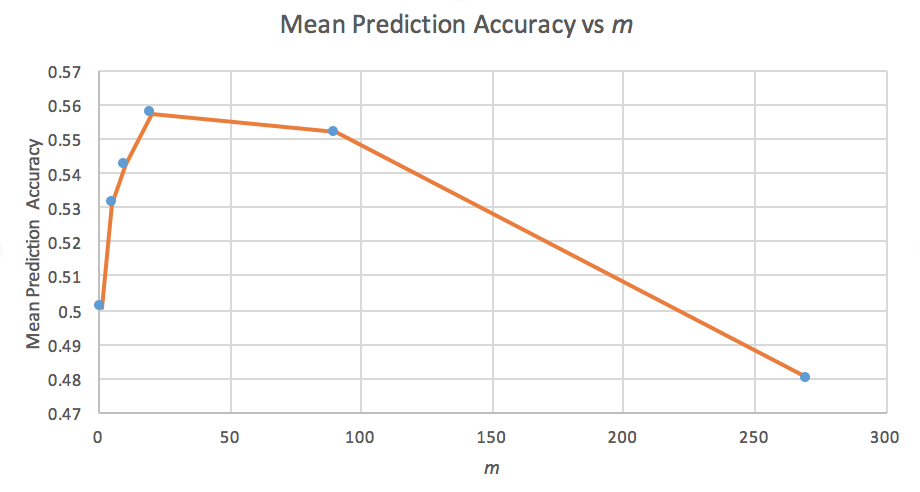
\includegraphics[width=0.9\textwidth]{MeanReturnvsM.png}
\caption{The mean prediction accuracy for each parameter $m$}
\label{fig: meanvsm}
\end{figure}

\newpage
This number does not tell the whole story, however. Looking at the full results in the Appendix, we see that when $m$ is small, varying $n_1$ and $n_2$ has little effect. For example, when $m=1$ the mean accuracy is within 49.5\% and 50.53\% for every combination of $n_1, n_2$. It is interesting to note that for prediction when $m=1$ very small values or very large values of $n_1, n_2$ work best. Mean and median accuracy are highest when at least one of the two is 5, or when both are 90 or 270. This implies that very short-term trends, or long-term trends, are best for predicting the next day's price direction. Trends across two weeks or a month, though, perform worse than simple random guessing.

The parameters $n_1$ and $n_2$ start to become more important as we increase $m$. When $m=10$ the mean prediction accuracy varies between 53.3\% and 56.8\%, a much larger range than at $m=1$. This disparity is exaggerated when $m=90$, that is, when we try to predict the price direction across the next quarter. Some combinations of $n_1, n_2$, such as $n_1=10, n_2=90$ actually result in less than 50\% accuracy, which means one would be better off flipping a coin, whereas other combinations have very high accuracies. For example, $n_1 = 270, n_2 = 5$ results in a 61.5\% prediction accuracy. 

Such discrepancies indicate that as the model tries to forecast farther into the future, the input parameters and historical data have drastically more influence. This again reinforces the EMH and the idea of stocks as a random walk. Regardless of the historical data used, short-term changes are difficult to predict, indicating that trends do not matter much in the short run, but may still offer some predictive ability. On the other hand, long-term changes are subject to seasonality and the trends discussed in \ref{subsec: stock}. With the right input data, the model can take advantage of these trends. If the training data reflects similar conditions to those in the test dataset, the model will have high predictive power. However, the wrong training dataset can skew the model and even lead to worse than 50\% prediction accuracy. Figure \ref{fig: meansforquarter} shows the prediction accuracies for each combination of $n_1, n_2$ when $m=90$.
\vspace{20pt}
\begin{figure}[htb]
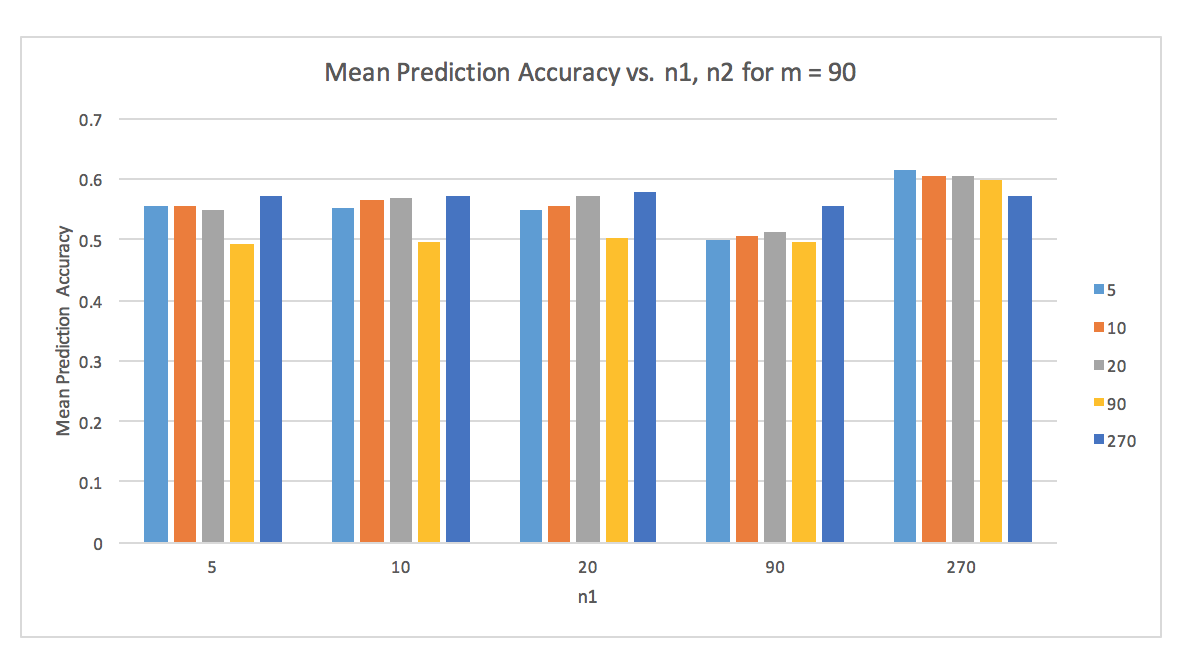
\includegraphics[width=0.9\textwidth]{MeanAccuraciesForQuarter.png}
\caption{The mean prediction accuracy for each combination of $n_1, n_2$ when $m=90$}
\label{fig: meansforquarter}
\end{figure}

\newpage
Another noticeable trend is that in general, $n_1 = 270$ results in the highest prediction accuracy for all $m$. That is, the overall sector’s historical data over the past year tends to be helpful in predicting the price direction at any point in the future. It is more helpful as we try to predict further into the future, but even in the short-term, it appears that the general sector trend is a better predictor than the short-term sector trend.

Almost the opposite is true for the parameter $n_2$. Mean prediction accuracy tends to be highest when $n_2 = 5$, the smallest value, but this is affected by parameter $m$. When $m$ is small too, choosing $n_2=5$ has most effect; when $m$ is small it still performs better than other values of $n_2$, but not as much.  This makes intuitive sense; a stock’s recent momentum is better than other indicators since it reflects most recent information. However, recent momentum is not as helpful when trying to predict farther into the future.

When $m$ is small, the choice of parameter $n_2$ has more effect than choice of parameter $n_1$, and here performance is best when $n_2 = 5$. As $m$ increases, the choice of parameter $n_1$ becomes more important. Again, this makes intuitive sense. When trying to predict price direction in the short term, the particular stock’s momentum can provide some indication (but not much). For predicting long-term price direction, the long-term sector trends are most helpful. Long-term sector trends reflect the market’s overall macro-conditions, and are not swayed by small fluctuations. The particular stock’s data, however, reflects only idiosyncratic conditions. This indicates that predicting long-term price direction for a particular stock might depend more on the overall market’s direction, and larger macro-conditions, than on the stock’s own trends. Once again, this supports EMH. If long-term stock direction were predictable based solely on that stock itself, this would mean prices react not only to new information but also to existing information, violating EMH.

It is also important to note that for short-term periods, simply being able to somewhat accurately predict tomorrow's price direction does not necessarily translate into trading profits. Treating the problem as binary classification allows us to more easily construct models, but it also means that we cannot predict the magnitude of the price change. Stock transactions have transaction costs, and the profit gained from small trades might not outweigh the costs.  Even though we did not find predictive ability for the next day, we were able to find some predictive ability within the next week or month. Nevertheless, translating this small predictive advantage into trading profits is entirely another issue.

Finally, we note that the long-term predictive ability also may not directly translate to long-term profits, although not due to trading costs. When $m=90, 270$ the overall mean predictive accuracy is less than in the short term, but with the right choice of parameters $n_1, n_2$ the accuracy can be higher than 60\%. This number is itself an average of the prediction accuracies for each of the 34. As discussed above and seen in the Appendix, the range of prediction for stocks increases as we increase $m$, and becomes very large when $m=90, 270$. We see that the model is able to predict price direction for some stocks with greater than 80\% accuracy, but for others cannot predict with more than 30\% accuracy. The problem is that we do not yet know ahead of time which stocks the model will be able to predict accurately and which it will not, so profiting off the model is still difficult without more experimentation.

\section{Future Work}
\subsection{Adding Granularity}
One limitation of this study is that we only looked at daily stock price data. As a result, our momentum and volatility parameters were calculated over weeks. This is different from actual hedge funds and quantitative trading institutions, which study price data at a far more granular level, on the order of minutes or even seconds. We can further this study by looking at intra-day trading data in addition to closing price data. By observing intra-day trends, we can create more robust models that capitalize on sudden changes in momentum during intra-day trading. Individual stocks often have price swings that last only for a couple minutes, which an intra-day model can analyze, and then use to predict price direction in the next few seconds or minutes. This is how such financial institutions make trading profits.

\subsection{Feature Selection}
Feature selection often has the biggest impact on a machine learning model’s accuracy. Another area for future work is to add to our feature list. Here we have looked at price volatility and momentum for the particular stock and for the technology sector. Future work would involve adding features related to the specific company and related to broader macroeconomic factors. Features related to the specific company include its Price/Earnings ratio, its market cap, working capital ratio, cost-of-capital, etc. Features related to broader factors include interest rate, inflation, GDP growth rate, etc.

\subsection{Analyzing Other Sectors and Sizes}
Another area for future growth is to apply our model to stocks in other sectors. In this study we have only focused on the technology sector, specifically 34 mature technology companies. We can apply our methods to other sectors such as healthcare, retail, service, etc. We can also apply our methods to mid-size and startup companies, to see how the size of a company affects our model’s predictive ability. 

\newpage
\section*{Appendix: Results Data}
\label{app: appendix}
Here we present the full data table of results.

% \begin{table}[H]
% \caption{Data showing prediction accuracy summary statistics for each combination of $m, n_1, n_2$}
\footnotesize
\begin{longtable}{p{2cm} p{2cm} p{2cm} p{2cm} p{2cm} p{2cm} p{2cm}}
\caption{Data showing prediction accuracy summary statistics for each combination of $m, n_1, n_2$} \\
\hline
$m$ & $n_1$ & $n_2$ & mean & median & max & min \\
\hline
% 1 & 5 & 5 & 0.5039 & 0.5086 & 0.5325 & 0.4714 \\
% & 5 & 10 & 0.5012 & 0.5020 & 0.5525 & 0.6588 \\
% & 5 & 20 & 0.5042 & 0.5080 & 0.5471 & 0.4635 \\
% & 5 & 90 & 0.5053 & 0.5086 & 0.5445 & 0.4595 \\
% & 5 & 270 & 0.5038 & 0.5073 & 0.5458 & 0.4635 \\ 
% & 10 & 5 & 0.4992 & 0.4967 & 0.5321 & 0.4679 \\
% & 10 & 10 & 0.4946 & 0.4940 & 0.5564 & 0.4568 \\
% & 10 & 20 & 0.4943 & 0.4980 & 

1 & 5 & 5 & 0.503945 & 0.508632 & 0.532537 & 0.471448 \\

& 5 & 10 & 0.501211 & 0.501992 & 0.552457 & 0.468792 \\

& 5 & 20 & 0.504179 & 0.507968 & 0.547145 & 0.463479 \\

& 5 & 90 & 0.505273 & 0.508632 & 0.544489 & 0.463479 \\

& 5 & 270 & 0.503828 & 0.507304 & 0.545817 & 0.459495 \\

& 10 & 5 & 0.499253 & 0.496658 & 0.532086 & 0.467914 \\

& 10 & 10 & 0.494571 & 0.494024 & 0.556441 & 0.456839 \\

& 10 & 20 & 0.494336 & 0.498008 & 0.545817 & 0.455511 \\

& 10 & 90 & 0.495508 & 0.499336 & 0.543161 & 0.438247 \\

& 10 & 270 & 0.498477 & 0.498008 & 0.540505 & 0.456839 \\

& 20 & 5 & 0.502909 & 0.503388 & 0.536585 & 0.471545 \\

& 20 & 10 & 0.498971 & 0.500000 & 0.557201 & 0.464334 \\

& 20 & 20 & 0.502578 & 0.505976 & 0.540505 & 0.443559 \\

& 20 & 90 & 0.499258 & 0.496016 & 0.543161 & 0.455511 \\

& 20 & 270 & 0.504726 & 0.511952 & 0.543161 & 0.456839 \\

& 90 & 5 & 0.500925 & 0.502246 & 0.532934 & 0.453593 \\

& 90 & 10 & 0.500568 & 0.502229 & 0.540862 & 0.453195 \\

& 90 & 20 & 0.499871 & 0.500732 & 0.543192 & 0.452416 \\

& 90 & 90 & 0.498984 & 0.495352 & 0.543161 & 0.456839 \\

& 90 & 270 & 0.503711 & 0.504648 & 0.543161 & 0.456839 \\

& 270 & 5 & 0.502712 & 0.509221 & 0.561475 & 0.461066 \\

& 270 & 10 & 0.495168 & 0.498986 & 0.553753 & 0.430020 \\

& 270 & 20 & 0.501696 & 0.501988 & 0.554672 & 0.425447 \\

& 270 & 90 & 0.500616 & 0.496510 & 0.541012 & 0.441536 \\

& 270 & 270 & 0.503437 & 0.506640 & 0.543161 & 0.456839 \\
\hline
5 & 5 & 5 & 0.523757 & 0.530708 & 0.618158 & 0.411215 \\

& 5 & 10 & 0.525053 & 0.530040 & 0.588785 & 0.452603 \\

& 5 & 20 & 0.528548 & 0.534713 & 0.579439 & 0.403204 \\

& 5 & 90 & 0.526310 & 0.529372 & 0.592790 & 0.401869 \\

& 5 & 270 & 0.530001 & 0.538051 & 0.598131 & 0.401869 \\

& 10 & 5 & 0.524984 & 0.524194 & 0.598118 & 0.419355 \\

& 10 & 10 & 0.521872 & 0.528037 & 0.588785 & 0.427236 \\

& 10 & 20 & 0.521165 & 0.528037 & 0.590120 & 0.403204 \\

& 10 & 90 & 0.515668 & 0.527370 & 0.596796 & 0.404539 \\

& 10 & 270 & 0.525563 & 0.534045 & 0.599466 & 0.404539 \\

& 20 & 5 & 0.531215 & 0.532698 & 0.588556 & 0.435967 \\

& 20 & 10 & 0.527700 & 0.535183 & 0.587280 & 0.441137 \\

& 20 & 20 & 0.533103 & 0.535381 & 0.610147 & 0.419226 \\

& 20 & 90 & 0.531061 & 0.536716 & 0.612817 & 0.380507 \\

& 20 & 270 & 0.540642 & 0.547397 & 0.612817 & 0.385848 \\

& 90 & 5 & 0.528792 & 0.526355 & 0.602410 & 0.403614 \\

& 90 & 10 & 0.525763 & 0.528401 & 0.596413 & 0.445441 \\

& 90 & 20 & 0.532617 & 0.536819 & 0.625920 & 0.387334 \\

& 90 & 90 & 0.529765 & 0.536048 & 0.598131 & 0.401869 \\

& 90 & 270 & 0.532828 & 0.546061 & 0.588785 & 0.401869 \\

& 270 & 5 & 0.548311 & 0.549587 & 0.607438 & 0.479339 \\

& 270 & 10 & 0.548178 & 0.550102 & 0.605317 & 0.449898 \\

& 270 & 20 & 0.549275 & 0.552104 & 0.607214 & 0.446894 \\

& 270 & 90 & 0.534736 & 0.549209 & 0.604569 & 0.363796 \\

& 270 & 270 & 0.540603 & 0.548064 & 0.615487 & 0.401869 \\
\hline
10 & 5 & 5 & 0.537200 & 0.540323 & 0.596774 & 0.452957 \\

& 5 & 10 & 0.539295 & 0.545027 & 0.602151 & 0.440860 \\

& 5 & 20 & 0.540283 & 0.545027 & 0.618280 & 0.375000 \\

& 5 & 90 & 0.540006 & 0.542339 & 0.610215 & 0.361559 \\

& 5 & 270 & 0.543683 & 0.548387 & 0.607527 & 0.376344 \\

& 10 & 5 & 0.536058 & 0.540595 & 0.595399 & 0.441137 \\

& 10 & 10 & 0.534472 & 0.549059 & 0.607527 & 0.438172 \\

& 10 & 20 & 0.535421 & 0.545699 & 0.622312 & 0.372312 \\

& 10 & 90 & 0.533286 & 0.538978 & 0.623656 & 0.380376 \\

& 10 & 270 & 0.544711 & 0.547715 & 0.603495 & 0.412634 \\

& 20 & 5 & 0.539377 & 0.544582 & 0.620027 & 0.441701 \\

& 20 & 10 & 0.540030 & 0.542234 & 0.632153 & 0.420981 \\

& 20 & 20 & 0.540560 & 0.545699 & 0.650538 & 0.381720 \\

& 20 & 90 & 0.541469 & 0.550403 & 0.618280 & 0.369624 \\

& 20 & 270 & 0.550166 & 0.555108 & 0.662634 & 0.373656 \\

& 90 & 5 & 0.539097 & 0.545524 & 0.603945 & 0.435508 \\

& 90 & 10 & 0.535746 & 0.537651 & 0.620482 & 0.405120 \\

& 90 & 20 & 0.535477 & 0.550445 & 0.637982 & 0.341246 \\

& 90 & 90 & 0.540639 & 0.545699 & 0.622312 & 0.380376 \\

& 90 & 270 & 0.539097 & 0.548387 & 0.615591 & 0.357527 \\

& 270 & 5 & 0.559069 & 0.557411 & 0.653445 & 0.427975 \\

& 270 & 10 & 0.556089 & 0.557851 & 0.652893 & 0.407025 \\

& 270 & 20 & 0.568052 & 0.571862 & 0.663968 & 0.374494 \\

& 270 & 90 & 0.549645 & 0.559397 & 0.643617 & 0.347518 \\

& 270 & 270 & 0.543169 & 0.552419 & 0.615591 & 0.357527 \\
\hline
20 & 5 & 5 & 0.553775 & 0.559946 & 0.658038 & 0.336512 \\

& 5 & 10 & 0.555658 & 0.566757 & 0.668937 & 0.331063 \\

& 5 & 20 & 0.550809 & 0.555177 & 0.686649 & 0.325613 \\

& 5 & 90 & 0.546642 & 0.564033 & 0.663488 & 0.325613 \\

& 5 & 270 & 0.568040 & 0.580381 & 0.653951 & 0.335150 \\

& 10 & 5 & 0.549827 & 0.551440 & 0.663923 & 0.336077 \\

& 10 & 10 & 0.557020 & 0.566757 & 0.688011 & 0.325613 \\

& 10 & 20 & 0.545560 & 0.555858 & 0.688011 & 0.324251 \\

& 10 & 90 & 0.545560 & 0.560627 & 0.664850 & 0.324251 \\

& 10 & 270 & 0.575373 & 0.581063 & 0.713896 & 0.322888 \\

& 20 & 5 & 0.554365 & 0.556328 & 0.671766 & 0.321280 \\

& 20 & 10 & 0.554802 & 0.558011 & 0.680939 & 0.325967 \\

& 20 & 20 & 0.548325 & 0.556540 & 0.697548 & 0.324251 \\

& 20 & 90 & 0.550128 & 0.574932 & 0.678474 & 0.324251 \\

& 20 & 270 & 0.567879 & 0.580381 & 0.664850 & 0.299728 \\

& 90 & 5 & 0.548491 & 0.565485 & 0.677966 & 0.302003 \\

& 90 & 10 & 0.552303 & 0.566514 & 0.689602 & 0.307339 \\

& 90 & 20 & 0.547263 & 0.564006 & 0.697289 & 0.311747 \\

& 90 & 90 & 0.546281 & 0.568801 & 0.667575 & 0.324251 \\

& 90 & 270 & 0.555698 & 0.577657 & 0.653951 & 0.324251 \\

& 270 & 5 & 0.572871 & 0.575693 & 0.705757 & 0.353945 \\

& 270 & 10 & 0.578369 & 0.580169 & 0.708861 & 0.373418 \\

& 270 & 20 & 0.573955 & 0.586777 & 0.714876 & 0.342975 \\

& 270 & 90 & 0.561319 & 0.596570 & 0.709386 & 0.296029 \\

& 270 & 270 & 0.570724 & 0.580381 & 0.679837 & 0.324251 \\
& & & & & & \\
\hline
90 & 5 & 5 & 0.555679 & 0.570030 & 0.849398 & 0.251506 \\

& 5 & 10 & 0.554571 & 0.545934 & 0.849398 & 0.256024 \\

& 5 & 20 & 0.550053 & 0.551205 & 0.849398 & 0.222892 \\

& 5 & 90 & 0.492470 & 0.491717 & 0.849398 & 0.203313 \\

& 5 & 270 & 0.572821 & 0.602410 & 0.814759 & 0.161145 \\

& 10 & 5 & 0.551415 & 0.562974 & 0.848255 & 0.239757 \\

& 10 & 10 & 0.565556 & 0.574548 & 0.849398 & 0.236446 \\

& 10 & 20 & 0.567328 & 0.588102 & 0.849398 & 0.201807 \\

& 10 & 90 & 0.497387 & 0.520331 & 0.849398 & 0.194277 \\

& 10 & 270 & 0.571536 & 0.597139 & 0.774096 & 0.165663 \\

& 20 & 5 & 0.549760 & 0.566256 & 0.852080 & 0.221880 \\

& 20 & 10 & 0.556845 & 0.563456 & 0.847095 & 0.244648 \\

& 20 & 20 & 0.570030 & 0.571536 & 0.849398 & 0.225904 \\

& 20 & 90 & 0.501329 & 0.516566 & 0.849398 & 0.167169 \\

& 20 & 270 & 0.577826 & 0.617470 & 0.796687 & 0.118976 \\

& 90 & 5 & 0.498324 & 0.524180 & 0.911917 & 0.138169 \\

& 90 & 10 & 0.504684 & 0.517123 & 0.912671 & 0.160959 \\

& 90 & 20 & 0.512280 & 0.520202 & 0.910774 & 0.173401 \\

& 90 & 90 & 0.495748 & 0.496988 & 0.849398 & 0.240964 \\

& 90 & 270 & 0.555679 & 0.576807 & 0.774096 & 0.259036 \\

& 270 & 5 & 0.614993 & 0.585213 & 0.939850 & 0.258145 \\

& 270 & 10 & 0.605926 & 0.602723 & 0.893564 & 0.118812 \\

& 270 & 20 & 0.604149 & 0.608696 & 0.915459 & 0.200483 \\

& 270 & 90 & 0.598991 & 0.596074 & 0.911157 & 0.123967 \\

& 270 & 270 & 0.571580 & 0.602410 & 0.774096 & 0.207831 \\
\hline
270 & 5 & 5 & 0.392076 & 0.331612 & 0.983471 & 0.000000 \\

& 5 & 10 & 0.390010 & 0.321281 & 0.985537 & 0.000000 \\

& 5 & 20 & 0.403804 & 0.376033 & 0.987603 & 0.000000 \\

& 5 & 90 & 0.389645 & 0.297521 & 0.971074 & 0.000000 \\

& 5 & 270 & 0.517076 & 0.482438 & 0.987603 & 0.010331 \\

& 10 & 5 & 0.397765 & 0.354906 & 0.987474 & 0.000000 \\

& 10 & 10 & 0.398213 & 0.354339 & 0.987603 & 0.000000 \\

& 10 & 20 & 0.408483 & 0.372934 & 0.987603 & 0.000000 \\

& 10 & 90 & 0.399003 & 0.317149 & 0.971074 & 0.000000 \\

& 10 & 270 & 0.514463 & 0.488636 & 0.987603 & 0.010331 \\

& 20 & 5 & 0.406434 & 0.373134 & 0.982942 & 0.006397 \\

& 20 & 10 & 0.415488 & 0.360759 & 0.985232 & 0.000000 \\

& 20 & 20 & 0.421123 & 0.387397 & 0.987603 & 0.000000 \\

& 20 & 90 & 0.413345 & 0.359504 & 0.971074 & 0.000000 \\

& 20 & 270 & 0.521269 & 0.491736 & 0.987603 & 0.022727 \\

& 90 & 5 & 0.444788 & 0.408521 & 1.000000 & 0.007519 \\

& 90 & 10 & 0.449840 & 0.474010 & 1.000000 & 0.000000 \\

& 90 & 20 & 0.461921 & 0.457729 & 0.997585 & 0.002415 \\

& 90 & 90 & 0.432547 & 0.358471 & 0.971074 & 0.004132 \\

& 90 & 270 & 0.526434 & 0.534091 & 0.987603 & 0.002066 \\

& 270 & 5 & 0.691244 & 0.705479 & 1.000000 & 0.027397 \\

& 270 & 10 & 0.687763 & 0.732143 & 1.000000 & 0.035714 \\

& 270 & 20 & 0.675214 & 0.713675 & 1.000000 & 0.047009 \\

& 270 & 90 & 0.674632 & 0.731908 & 1.000000 & 0.111842 \\

& 270 & 270 & 0.568000 & 0.621901 & 0.987603 & 0.008264 \\
\hline
\end{longtable}
% \end{table}

\newpage
\bstctlcite{bstctl:etal, bstctl:nodash, bstctl:simpurl}
\bibliographystyle{IEEEtranS}
\bibliography{references}

\end{document}

